\begin{figure*}[!hbt]
  \centering
  \subfigure[Relative runtime with varying Frontier tolerance $\tau_f$]{
    \label{fig:adjust-frontier--runtime}
    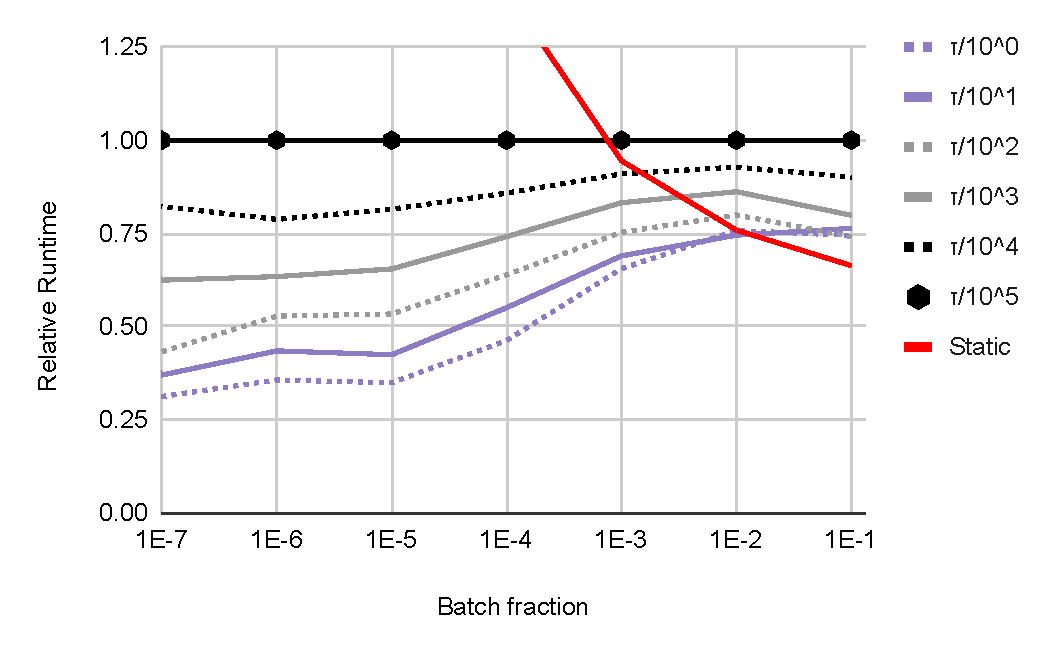
\includegraphics[width=0.48\linewidth]{out/adjust-frontier-runtime.pdf}
  }
  \subfigure[Error in ranks obtained with varying Frontier tolerance $\tau_f$]{
    \label{fig:adjust-frontier--error}
    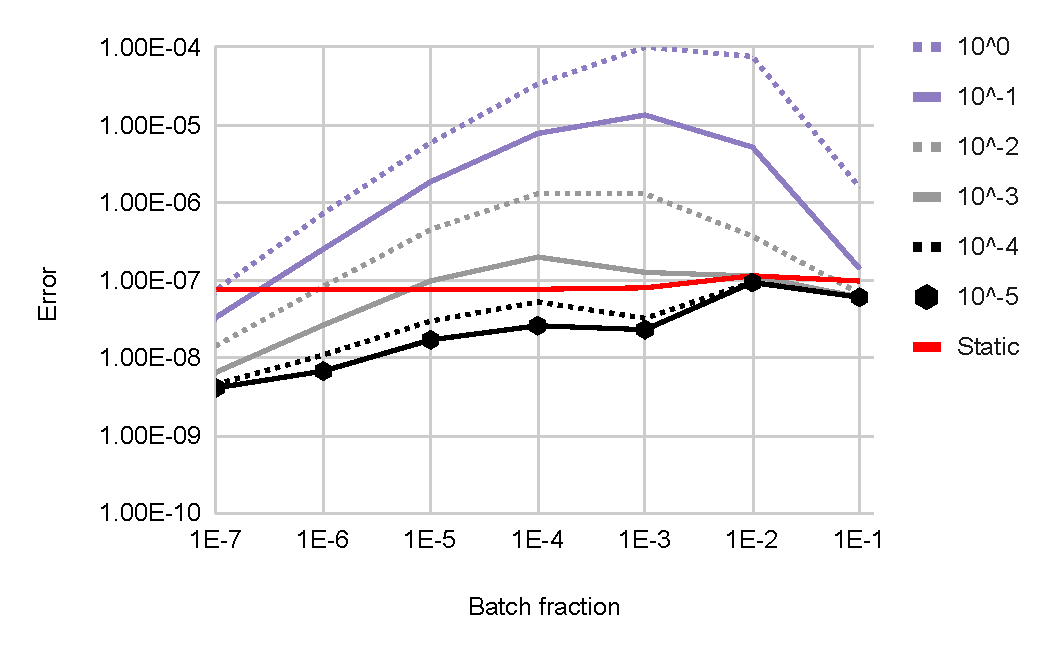
\includegraphics[width=0.48\linewidth]{out/adjust-frontier-error.pdf}
  } \\[-2ex]
  \caption{Average Relative runtime and Error in ranks obtained (with respect to ranks obtained with Reference Static PageRank) using \textit{Dynamic Frontier} approach, with frontier tolerance $\tau_f$ varying from $\tau$ to $\tau / 10^5$, on batch updates of size $10^{-7}|E|$ to $0.1|E|$. The figures indicate that increasing $\tau_f$ reduces runtime, but also increases the error. A Frontier tolerance $\tau_f$ of $\tau/10^4$ and $\tau/10^5$ obtain ranks with error lower than \textit{Static} PageRank, and are thus acceptable (we choose $\tau_f = \tau/10^5$ to be on the safe side).}
  \label{fig:adjust-frontier}
\end{figure*}
